\documentclass[12pt,a4paper]{article}
\usepackage[utf8]{inputenc}
\usepackage[spanish]{babel}
\usepackage[T1]{fontenc}
\usepackage{tocbibind} % Bibliografía en el indice
\usepackage{titlesec} % Posibilidad de editar los formatos de chapter
\usepackage{amsmath,amssymb,mathrsfs} % Matemáticas varias
\usepackage{siunitx} % SI de medidas
\usepackage{tabularx} % Para las tablas
\usepackage[title]{appendix} % Para anexos
\usepackage[spanish]{babel} % Para modificar labels por defecto
\renewcommand{\baselinestretch}{1} % Interlineado. 1 es estandar
% --- Arreglos varios para la inclusion de imagenes
\usepackage{float}
\usepackage[pdftex]{graphicx}
\usepackage{subfigure}
\usepackage{graphicx}
\graphicspath{{T:/Tom/Facultad/Logos/}{T:/Tom/Facultad/Materias/EDII/TPs/LED/Imagenes/}}
\usepackage[usenames,dvipsnames]{color}
\DeclareGraphicsExtensions{.png,.jpg,.pdf,.mps,.gif,.bmp}
% --- Para las dimensiones de los márgenes etc
\frenchspacing \addtolength{\hoffset}{-1.5cm}
\addtolength{\textwidth}{3cm} \addtolength{\voffset}{-2.5cm}
\addtolength{\textheight}{4cm}
% --- Para el encabezado
\setlength{\headheight}{33pt}
\usepackage{fancyhdr}
\fancyhead[R]{\includegraphics[height=1cm]{logo_fcefyn_nuevo.jpg}}\fancyhead[L]{\includegraphics[height=1cm]{unc1_a.jpg}}\fancyhead[C]{Electrónica Digital II} \fancyfoot[C]{Página \thepage} \renewcommand{\footrulewidth}{0.4pt}
\pagestyle{fancy}
% --- Para las tablas
\usepackage{multirow} % Juntar filas
\newcolumntype{L}[1]{>{\raggedright\arraybackslash}p{#1}} % Justificar Izq
\newcolumntype{C}[1]{>{\centering\arraybackslash}p{#1}} % Justificar Centrar
\newcolumntype{R}[1]{>{\raggedleft\arraybackslash}p{#1}} % Justificar Der
\usepackage[numbered]{bookmark} % Para que figure las secciones en el PDF
\usepackage{listings} % Para poner código 
\usepackage{enumitem} % Para editar las propiedades de los items
\usepackage{color}
\usepackage[bottom]{footmisc} % Para las notas al pie de la página
\lstset{frame=single} % Código en un cuadro
% --- Para Anexo
\addto\captionsspanish{%
  \renewcommand\appendixname{ANEXO}
  \renewcommand\appendixpagename{ANEXOS}
}
% -------------------------------------------------------- %
% Definicion de colores para el codigo
\lstdefinelanguage{XML}
{
  basicstyle=\ttfamily\footnotesize,
  morestring=[b]",
  moredelim=[s][\bfseries\color{Maroon}]{<}{\ },
  moredelim=[s][\bfseries\color{Maroon}]{</}{>},
  moredelim=[l][\bfseries\color{Maroon}]{/>},
  moredelim=[l][\bfseries\color{Maroon}]{>},
  morecomment=[s]{<?}{?>},
  morecomment=[s]{<!--}{-->},
  commentstyle=\color{DarkOliveGreen},
  stringstyle=\color{blue},
  identifierstyle=\color{red}
}

\renewcommand{\lstlistingname}{Código}

% -------------------------------------------------------- %

\begin{document}

\begin{titlepage}
    \begin{center}
        \vspace*{1cm}
        
        \Large
        \textbf{Universidad Nacional de Córdoba\\
        		Facultad de Ciencias Exatas, Físicas y Naturales}
        
        \vspace{0.5cm}
        \includegraphics[width=0.5\textwidth]{logo_caratula.png}
        
        \vspace{1.5cm}
        
        \textbf{Trabajo Práctico Final}\\
        Electrónica Digital II\\
        Docente: Ing. Martín Del Barco
        
        \vfill  
        
        \vspace{0.8cm}
        

        
        \Large
        Losano Quintana, Juan Cruz\\
        Piñero, Tomás Santiago\\
        Ingeniería en Computación\\
        Año 2019\\
        
        
    \end{center}
\end{titlepage}
% -------------------------------------------------------- %

% --- Tabla de contenidos

\setcounter{secnumdepth}{1}
\setcounter{tocdepth}{4}
\tableofcontents

% -------------------------------------------------------- %

\newpage
\renewcommand{\baselinestretch}{1}
\setlength{\parskip}{0.5em}

\section{Enunciado}



\section{Introducción}


\section{Desarrollo}
\subsection{Cálculos de resistencias}
	
\subsubsection{Pull-ups}

\subsubsection{LEDs}

\section{Implementación}
	El PIC tiene como frecuencia de reloj un cristal de \SI{4}{\MHz}, por lo que el ciclo de instrucción se realiza con una frecuencia de \SI{1}{\MHz} debido a que cada 4 ciclos del reloj se realiza una instrucción. Esto se debe a que para ejecutar la instrucción indicada, el PIC debe ejecutar cuatro acciones: 
	
	\begin{enumerate}[leftmargin=1.5cm,nosep]
	\item Buscar la instrucción en la memoria principal.
	\item Decodificar la instrucción.
	\item Ejecutar la instrucción.
	\item Almacenar los resultados.
	\end{enumerate}
	
	Esto es importante para el cálculo de la subrutina de retardo, ya que depende de la frecuencia de reloj que se utilice.
	
	A continuación se muestran los diagramas de flujo del programa utilizado.
	
\subsection{Diagramas de flujo}
	En esta sección se muestran los diagramas de flujo del programa principal y las subrutinas que utiliza.
	
	\subsubsection{Programa principal}	
	Primero se realiza la configuración de los puertos A y B como salida y entrada digitales, respectivamente. 
	
	Una vez configurados los puertos se toman los datos del puerto de entrada y a esa lectura se la invierte, ya que cuando los Dip Switch estén bajos las entradas estarán con un valor de uno lógico debido a la presencia de las resistencias pull-up.
	
	Consecuentemente el programa almacena los últimos cuatro bits en la variable \emph{numero1} y se lo suma a los primeros cuatro bits leídos, mostrando el resultado en los LEDs de salida. Si el resultado es de cinco bits, el LED del \emph{digit carry} parpadeará y no se podrá realizar otra suma hasta que se resetee el PIC.
	
%	\begin{figure}[H]
%	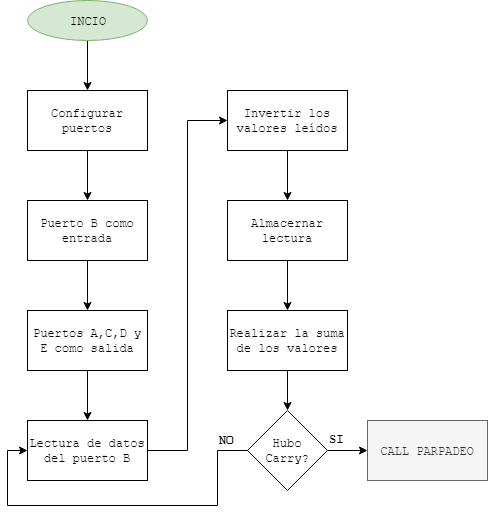
\includegraphics[scale=0.5]{programa.png}
%	\centering
%	\caption{Diagrama de flujo del programa.}
%	\end{figure}		
	
	\subsubsection{Parpadeo}

	\subsubsection{Delay}

\section{Esquema del circuito}

%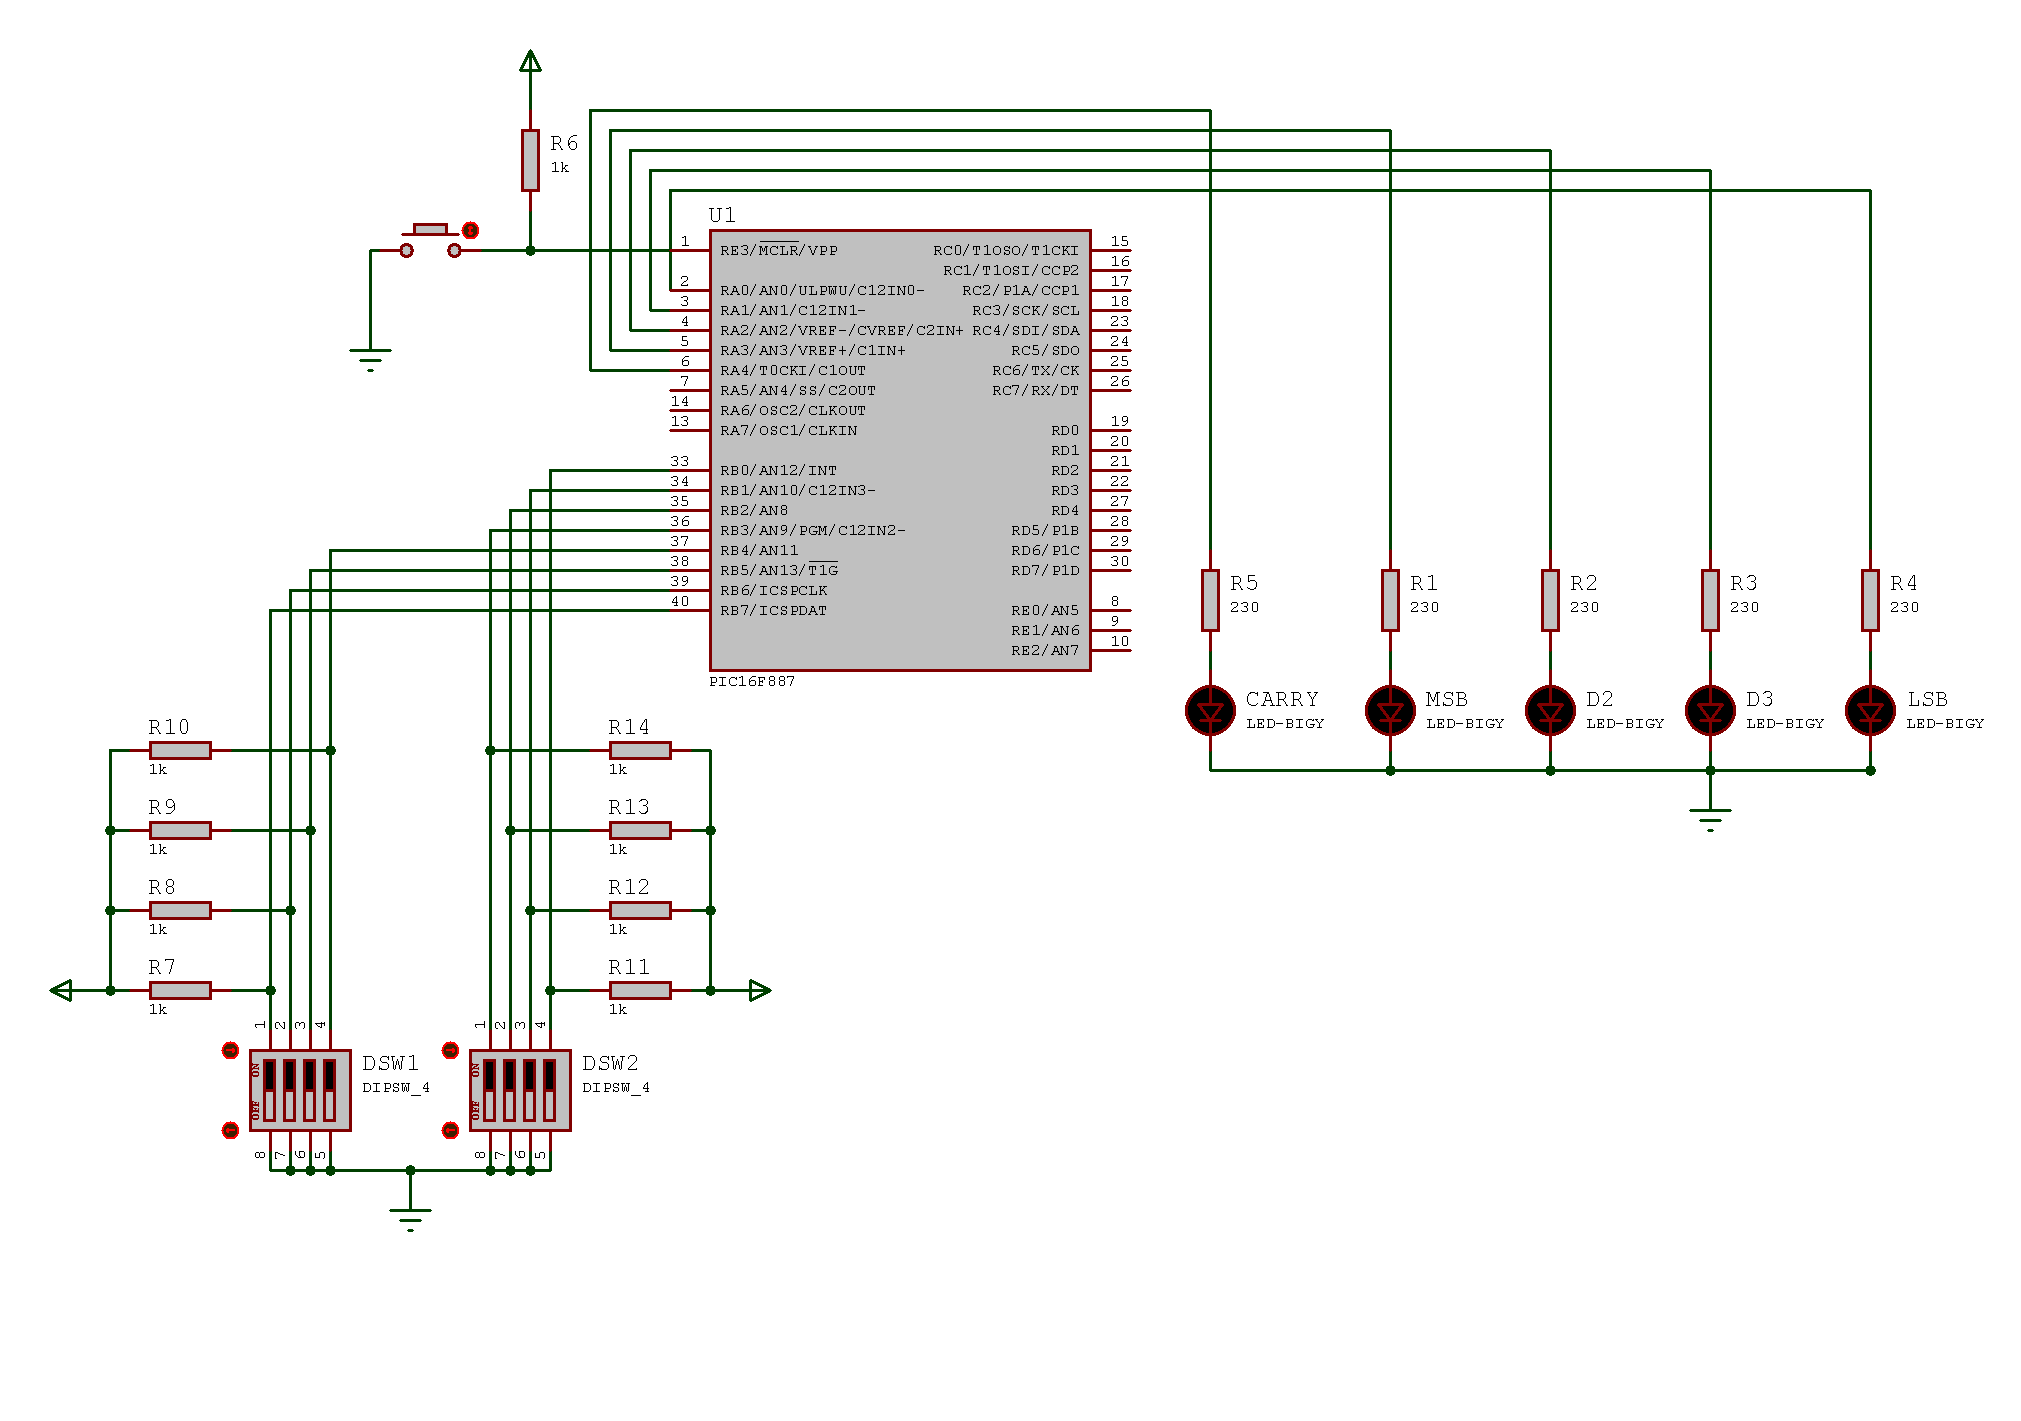
\includegraphics[angle=90,origin=c,scale=0.33]{circuito.png}
	
\end{document}